\documentclass[UTF8,aspectratio=169,10pt]{ctexbeamer}

\usetheme{Madrid}
\usecolortheme{default}
\usefonttheme{professionalfonts}

\usepackage{amsmath,amssymb,bm}
\usepackage{graphicx}
\usepackage{booktabs}
\usepackage{tikz}
\usetikzlibrary{positioning}
\usepackage{xcolor}
\usepackage{newtxmath}
\usepackage{fontspec}

\setmainfont{Times New Roman}
\setsansfont{Arial}
\setmonofont{Consolas}

\graphicspath{
  {../assets/}
  {../assets/q3_visualization/}
  {../assets/q3_comparison/}
  {../assets/q3_fem/}
}

\definecolor{tjublue}{RGB}{0,74,132}
\definecolor{tjuaccent}{RGB}{180,58,72}
\definecolor{softgray}{RGB}{245,247,250}

\setbeamercolor{palette primary}{bg=tjublue,fg=white}
\setbeamercolor{palette secondary}{bg=tjublue!85,fg=white}
\setbeamercolor{palette tertiary}{bg=tjublue!70,fg=white}
\setbeamercolor{frametitle}{bg=tjublue,fg=white}
\setbeamercolor{title}{fg=tjublue}
\setbeamercolor{block title}{bg=tjublue,fg=white}
\setbeamercolor{block body}{bg=softgray,fg=black}
\setbeamercolor{alerted text}{fg=tjuaccent}
\setbeamertemplate{navigation symbols}{}
\setbeamertemplate{caption}[numbered]

\newcommand{\keypoint}[1]{\begin{block}{要点}#1\end{block}}
\newcommand{\takeaway}[1]{\vfill{\small\color{tjublue}#1}}

\title[结构动力学 Q3]{带集中质量与局部弹簧支承 Euler--Bernoulli 梁自由振动的解析解与有限元验证}
\author{王子传 \quad 吕天翔 \quad 方思哲}
\institute{天津大学机械工程学院}
\date{}

\begin{document}

% 1
\begin{frame}
  \vspace{0.2em}
  \begin{beamercolorbox}[wd=\linewidth,rounded=true,shadow=true,sep=1.0em,center]{frametitle}
    {\Large\bfseries 带集中质量与局部弹簧支承 Euler--Bernoulli 梁自由振动的\\[0.25em]解析解与有限元验证}
  \end{beamercolorbox}
  \vspace{1.2em}
  \begin{center}
    {\large 王子传 \quad 吕天翔 \quad 方思哲}\\[0.8em]
    天津大学机械工程学院\\[2.5em]
    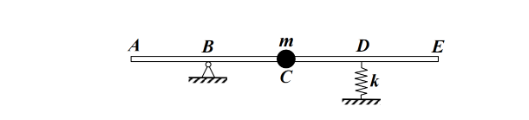
\includegraphics[width=0.48\linewidth]{image-20260616001638017.png}
  \end{center}
\end{frame}

% 2
\begin{frame}{汇报内容}
  \begin{columns}[T,onlytextwidth]
    \column{0.52\linewidth}
    \begin{enumerate}
      \item 研究背景与问题描述
      \item 解析解建模与推导
      \item 有限元模型与 Fortran 实现
      \item 解析解与 FEM 结果对比
      \item 结论与展望
    \end{enumerate}
    \column{0.42\linewidth}
    \begin{block}{主线}
      \[
      \text{问题建模}\rightarrow
      \text{解析求解}\rightarrow
      \text{数值验证}
      \]
    \end{block}
  \end{columns}
  \takeaway{先说明做什么，再说明怎么算，最后说明结果是否可信。}
\end{frame}

% 3
\begin{frame}{研究背景}
  \begin{itemize}
    \item 梁结构是机械、土木、航空航天和交通装备中的典型承载构件。
    \item 局部支承、附加质量、弹簧连接会显著改变结构动力特性。
    \item 含局部离散构件的连续梁需要同时进行解析建模和数值验证。
  \end{itemize}
  \vspace{0.8em}
  \begin{block}{核心关注}
    \[
    \text{局部约束/集中质量/弹簧支承}
    \Longrightarrow
    \text{固有频率、振型、动力响应变化}
    \]
  \end{block}
  \takeaway{本问题不是标准梁，而是连续梁与离散构件耦合的振动问题。}
\end{frame}

% 4
\begin{frame}{研究对象}
  \begin{columns}[T,onlytextwidth]
    \column{0.48\linewidth}
    \begin{itemize}
      \item 均质等截面 Euler--Bernoulli 梁
      \item 总长 $4l$，且 $AB=BC=CD=DE=l$
      \item $B$ 点为外部铰支座
      \item $C$ 点附加集中质量 $m$
      \item $D$ 点连接竖向线性弹簧 $k$
      \item 初始时刻 $C$ 点具有横向速度 $v_0$
    \end{itemize}
    \column{0.48\linewidth}
    \centering
    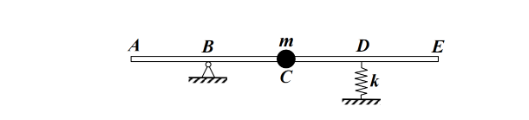
\includegraphics[width=\linewidth]{image-20260616001638017.png}
  \end{columns}
  \takeaway{$B$ 点是梁上的外部简单支承，不是梁内铰。}
\end{frame}

% 5
\begin{frame}{研究目标}
  \begin{columns}[T,onlytextwidth]
    \column{0.45\linewidth}
    \begin{block}{待求量}
      \begin{enumerate}
        \item 固有频率 $\omega_n$
        \item 振型函数 $\phi_n(x)$
        \item 初始速度作用下的动力响应 $w(x,t)$
        \item 解析解与 FEM 的一致性
      \end{enumerate}
    \end{block}
    \column{0.5\linewidth}
    \begin{block}{技术路线}
      \[
      \text{传递矩阵法}
      +\text{梁有限元法}
      +\text{后处理对比}
      \]
    \end{block}
  \end{columns}
  \takeaway{解析解提供理论基准，有限元法提供工程化验证。}
\end{frame}

% 6
\begin{frame}{基本假设}
  \begin{itemize}
    \item 梁满足 Euler--Bernoulli 梁理论。
    \item 材料线弹性、小变形。
    \item 梁为均质等截面。
    \item 集中质量只提供横向惯性。
    \item 弹簧为线性竖向弹簧。
    \item $B$ 点支座只约束竖向位移，不约束转角。
  \end{itemize}
  \begin{alertblock}{边界条件关键说明}
    \[
    B\text{ 点为连续梁上的外部简单支承点，而非梁内铰。}
    \]
  \end{alertblock}
\end{frame}

% 7
\begin{frame}{控制方程}
  \begin{block}{Euler--Bernoulli 梁段方程}
    \[
    \mu=\rho S,\qquad
    EJ\frac{\partial^4 w}{\partial x^4}
    +\rho S\frac{\partial^2 w}{\partial t^2}=0
    \]
  \end{block}
  \begin{block}{分离变量}
    \[
    w(x,t)=\phi(x)q(t),
    \qquad
    \phi^{(4)}-\lambda^4\phi=0
    \]
  \end{block}
  \takeaway{这是解析解的起点，后续边界和跳跃条件都作用在空间方程上。}
\end{frame}

% 8
\begin{frame}{无量纲化}
  \begin{columns}[T,onlytextwidth]
    \column{0.48\linewidth}
    \[
    \xi=\frac{x}{l}
    \]
    \[
    A:0,\quad B:1,\quad C:2,\quad D:3,\quad E:4
    \]
    \[
    \beta=\lambda l
    \]
    \column{0.48\linewidth}
    \begin{block}{无量纲空间方程}
      \[
      Y''''-\beta^4Y=0
      \]
    \end{block}
    \begin{block}{频率恢复}
      \[
      \omega_n=
      \frac{\beta_n^2}{l^2}
      \sqrt{\frac{EJ}{\rho S}}
      \]
    \end{block}
  \end{columns}
  \takeaway{求解的关键变为寻找特征根 $\beta_n$。}
\end{frame}

% 9
\begin{frame}{边界条件}
  \begin{columns}[T,onlytextwidth]
    \column{0.48\linewidth}
    \begin{block}{自由端 $A,E$}
      \[
      Y''(0)=Y'''(0)=0
      \]
      \[
      Y''(4)=Y'''(4)=0
      \]
    \end{block}
    \column{0.48\linewidth}
    \begin{block}{$B$ 点铰支}
      \[
      Y(1)=0
      \]
      \begin{itemize}
        \item $Y,Y',Y''$ 连续
        \item $Y'''$ 可因支座反力跳跃
      \end{itemize}
    \end{block}
  \end{columns}
  \takeaway{自由端对应弯矩和剪力为零；$B$ 点只约束位移。}
\end{frame}

% 10
\begin{frame}{集中质量与弹簧跳跃条件}
  \begin{columns}[T,onlytextwidth]
    \column{0.48\linewidth}
    \begin{block}{$C$ 点集中质量}
      \[
      Y'''(2^+)-Y'''(2^-)
      =\alpha\beta^4Y(2)
      \]
      \[
      \alpha=\frac{m}{\rho Sl}
      \]
    \end{block}
    \column{0.48\linewidth}
    \begin{block}{$D$ 点竖向弹簧}
      \[
      Y'''(3^+)-Y'''(3^-)
      =-\kappa Y(3)
      \]
      \[
      \kappa=\frac{kl^3}{EJ}
      \]
    \end{block}
  \end{columns}
  \takeaway{集中质量引入频率相关跳跃，弹簧引入位移相关跳跃。}
\end{frame}

% 11
\begin{frame}{传递矩阵法}
  \begin{block}{状态向量}
    \[
    \mathbf z(\xi)=
    \begin{bmatrix}
    Y & Y' & Y'' & Y'''
    \end{bmatrix}^{T}
    \]
  \end{block}
  \begin{columns}[T,onlytextwidth]
    \column{0.48\linewidth}
    \[
    \mathbf z(\xi+s)=\mathbf P(s)\mathbf z(\xi)
    \]
    \column{0.48\linewidth}
    \[
    \mathbf z(2^+)=\mathbf J_m\mathbf z(2^-)
    \]
    \[
    \mathbf z(3^+)=\mathbf J_k\mathbf z(3^-)
    \]
  \end{columns}
  \takeaway{梁段传递与局部跳跃统一到状态向量框架中。}
\end{frame}

% 12
\begin{frame}{频率方程}
  \begin{columns}[T,onlytextwidth]
    \column{0.48\linewidth}
    \begin{block}{左端自由状态}
      \[
      \mathbf z(0)=
      \begin{bmatrix}
      a & b & 0 & 0
      \end{bmatrix}^{T}
      \]
      \[
      \mathbf c=
      \begin{bmatrix}
      a & b & R
      \end{bmatrix}^{T}
      \]
    \end{block}
    \column{0.48\linewidth}
    \begin{block}{特征方程}
      \[
      \mathbf A(\beta)\mathbf c=\mathbf 0
      \]
      \[
      \det \mathbf A(\beta)=0
      \]
    \end{block}
  \end{columns}
  \takeaway{非平凡解条件给出特征根 $\beta_n$，进而得到固有频率。}
\end{frame}

% 13
\begin{frame}{解析特征根可视化}
  \begin{columns}[T,onlytextwidth]
    \column{0.62\linewidth}
    \centering
    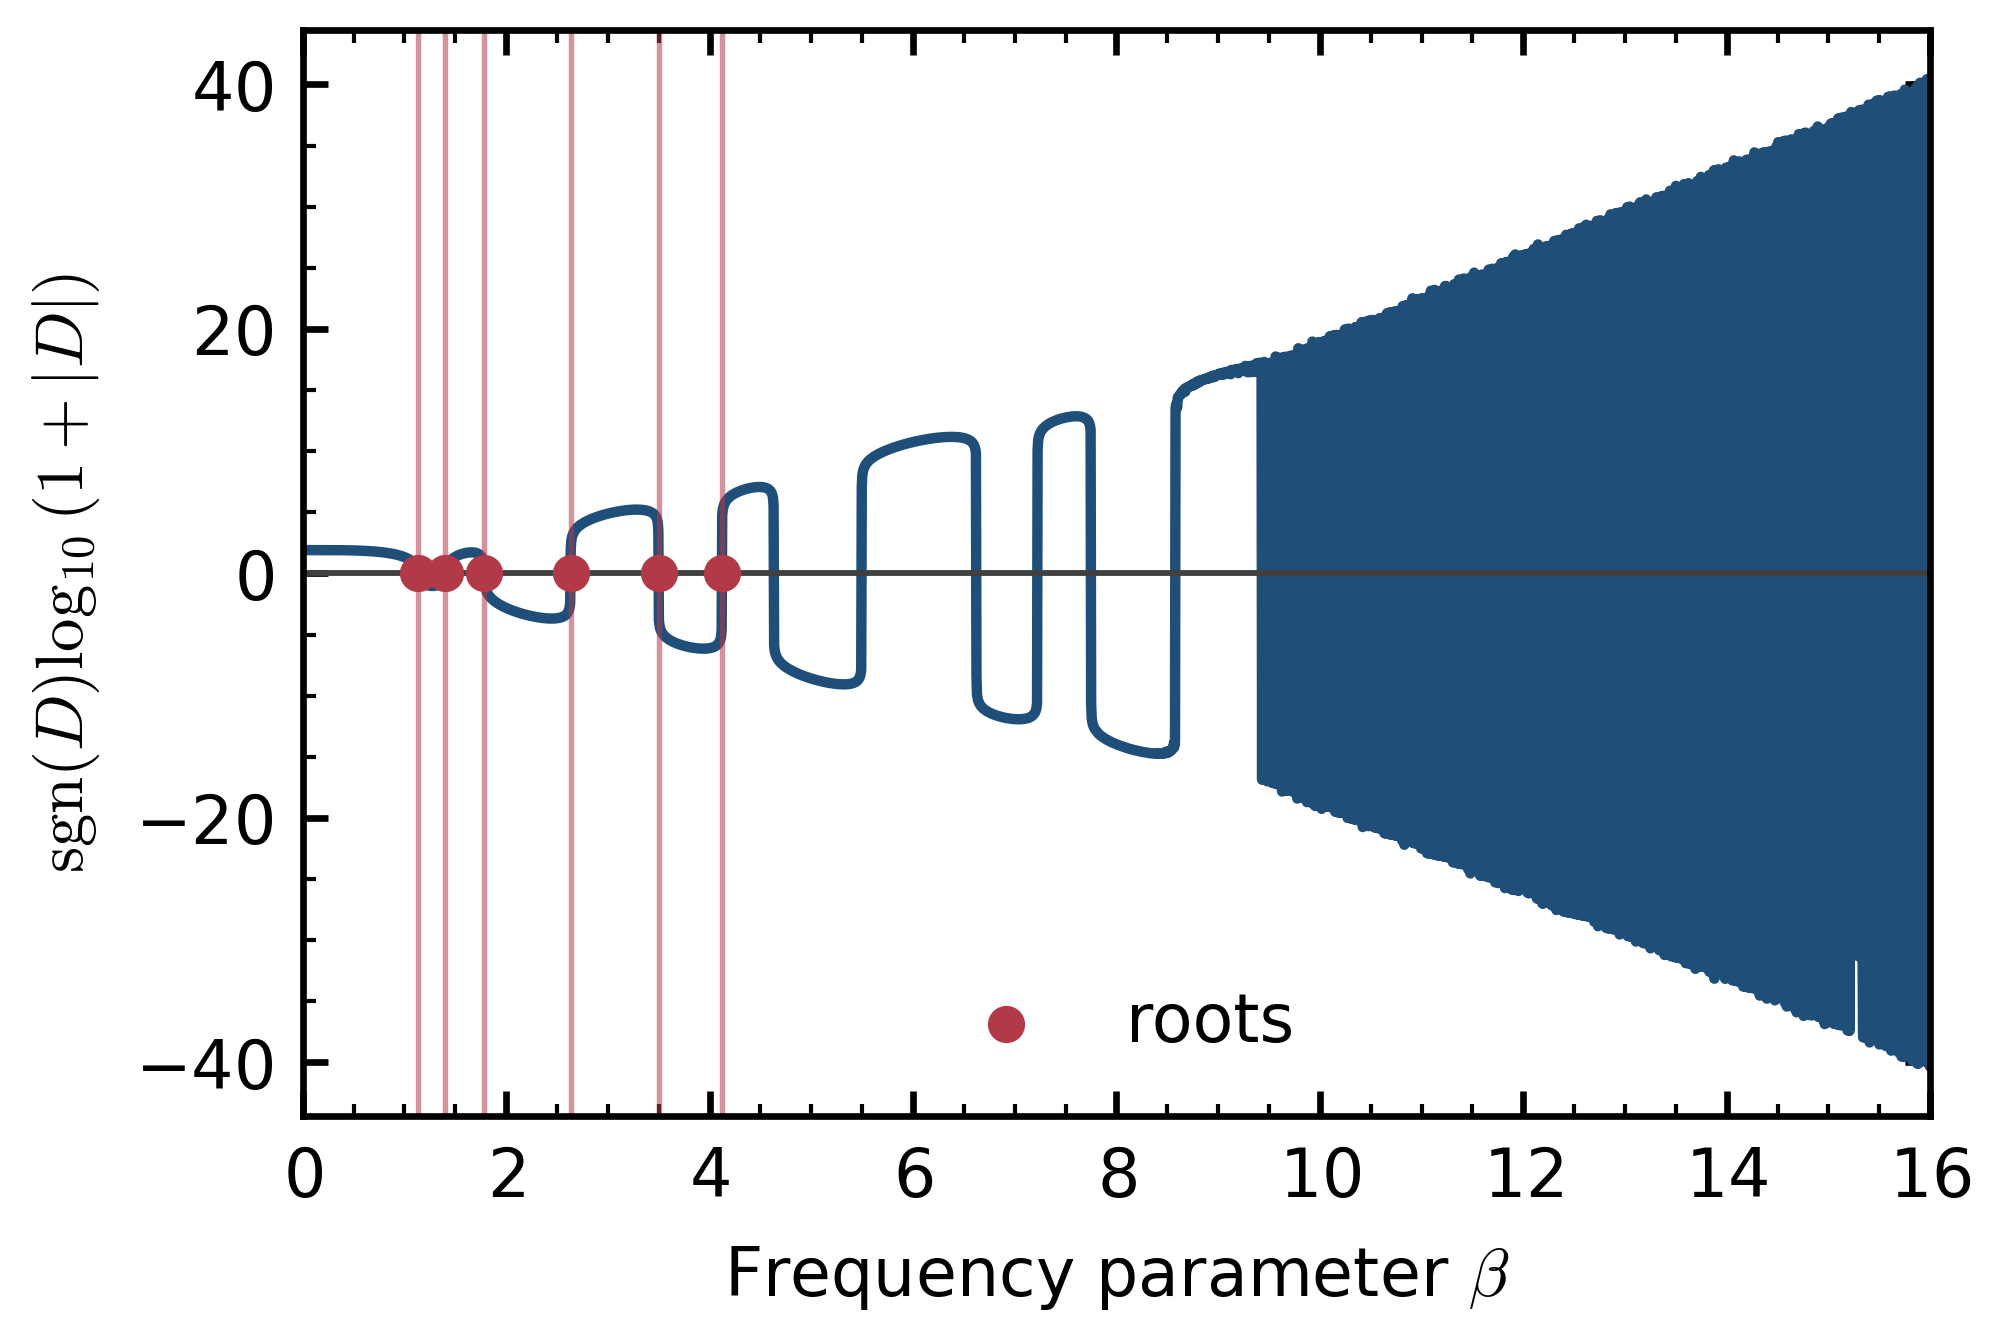
\includegraphics[width=\linewidth]{q3_characteristic_roots.png}
    \column{0.34\linewidth}
    \begin{itemize}
      \item 红色点为特征根位置
      \item $\bar{\omega}_n=\beta_n^2$
      \item 低阶根分布清晰
      \item 高阶区域振荡增强
    \end{itemize}
  \end{columns}
  \takeaway{解析解已经完成数值求根和可视化。}
\end{frame}

% 14
\begin{frame}{解析振型函数}
  \centering
  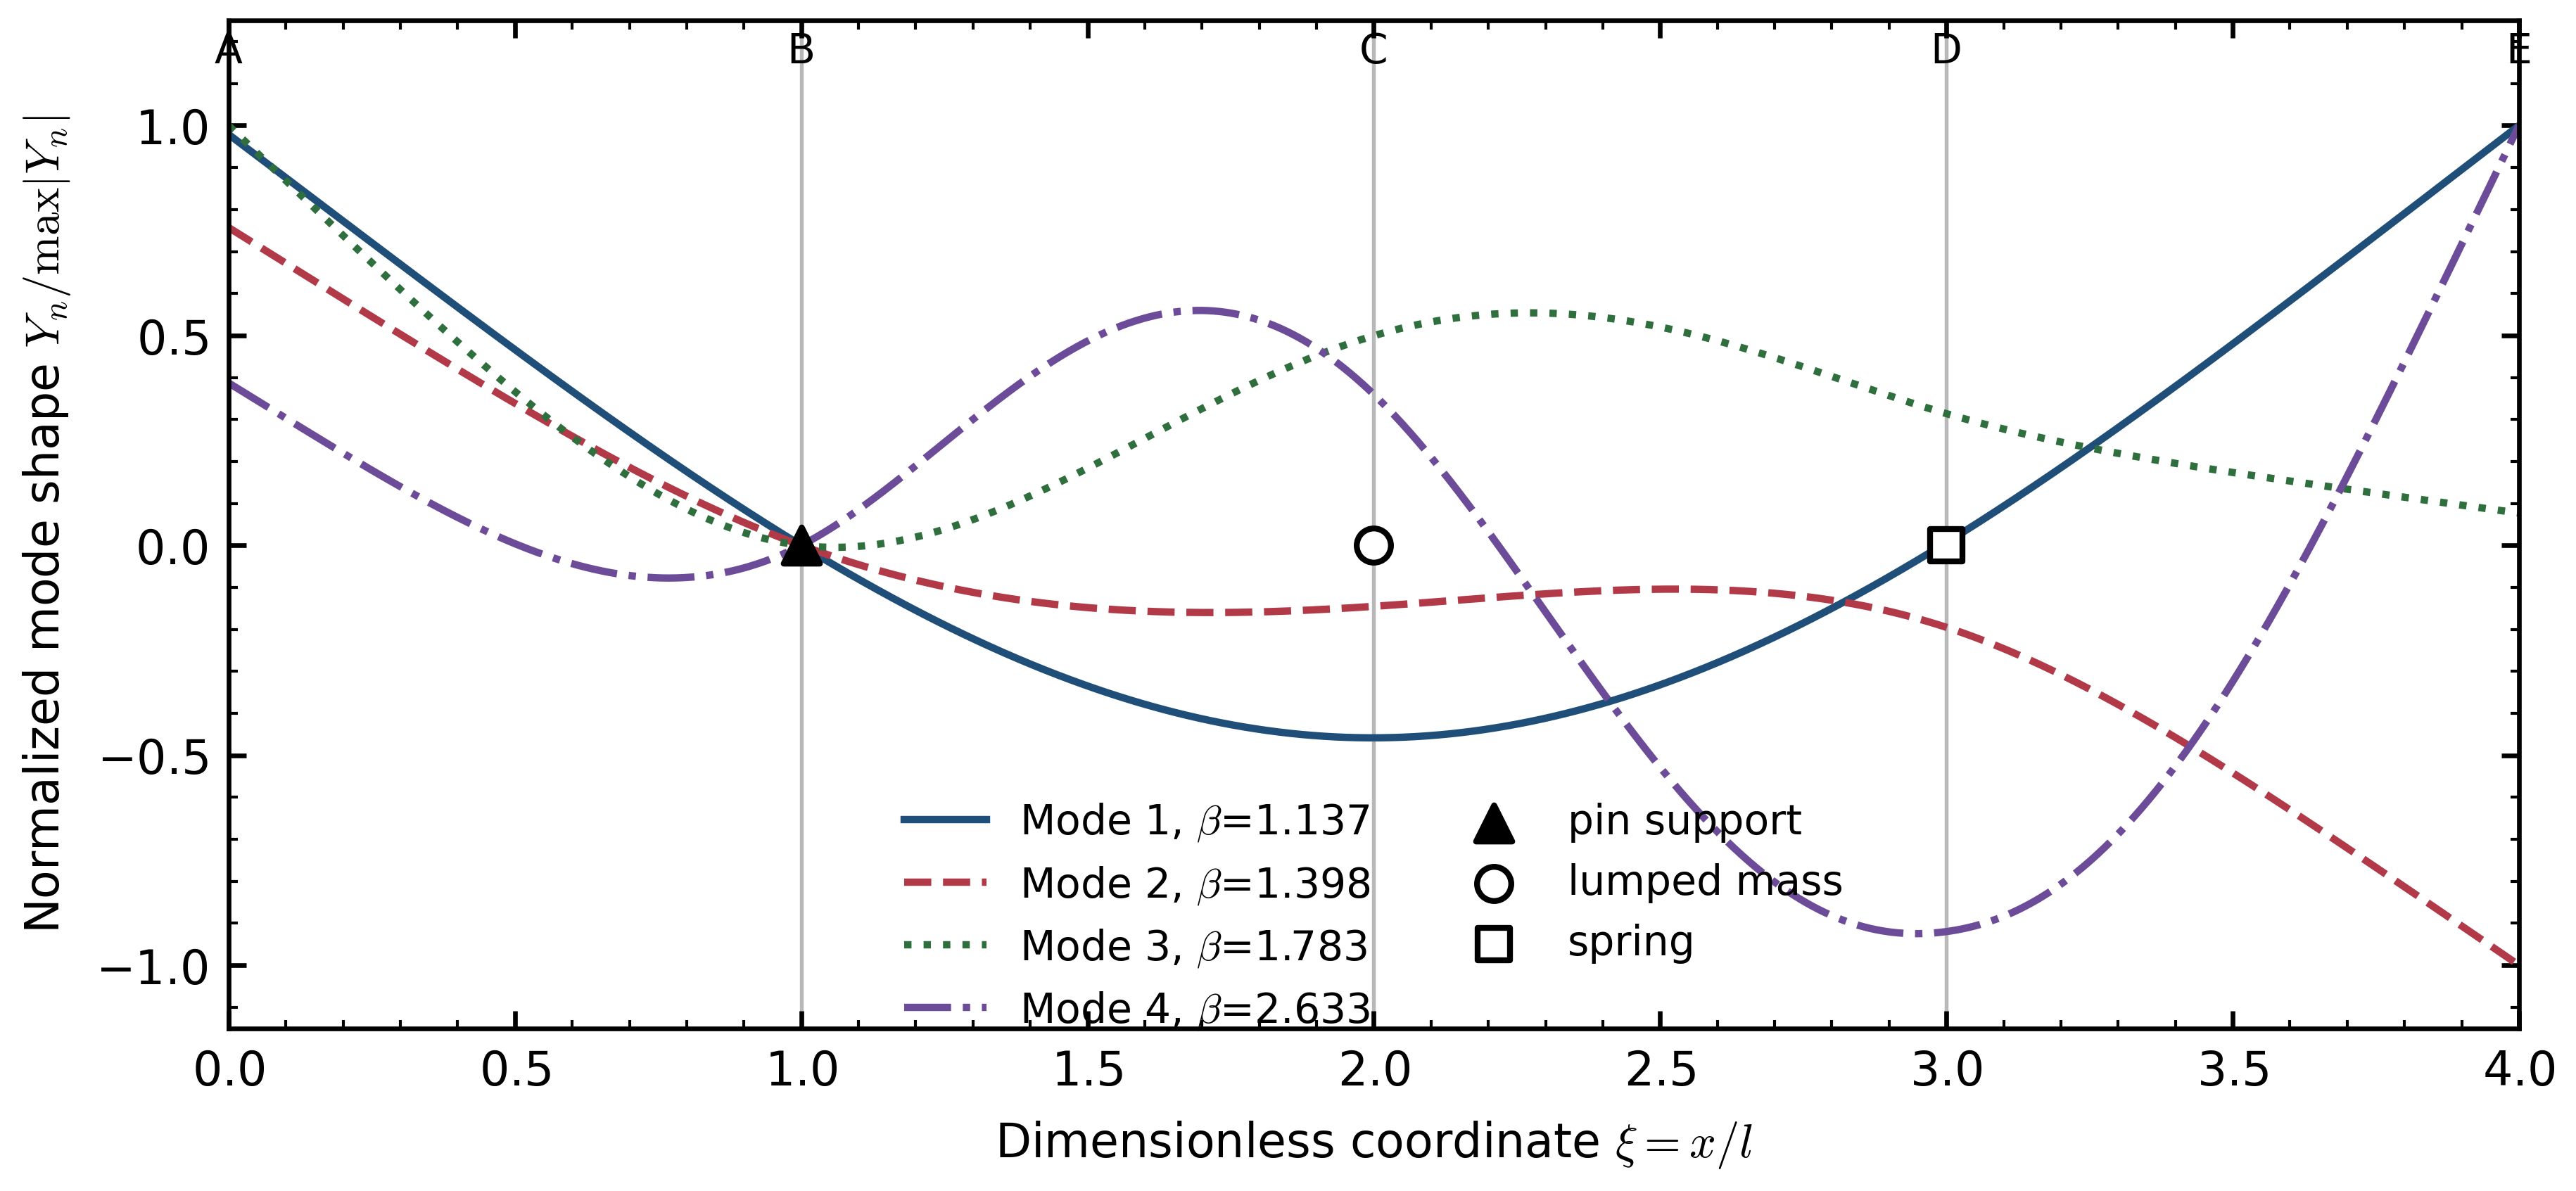
\includegraphics[width=0.82\linewidth]{q3_mode_shapes.png}
  \begin{itemize}
    \item $B$ 点位移为零，满足支承约束。
    \item $C,D$ 点位移连续，剪力通过跳跃条件反映局部构件作用。
  \end{itemize}
\end{frame}

% 15
\begin{frame}{解析动力响应}
  \begin{columns}[T,onlytextwidth]
    \column{0.43\linewidth}
    \begin{block}{模态响应}
      \[
      w(x,t)=
      \sum_{n=1}^{\infty}
      \phi_n(x)
      \frac{m v_0\phi_n(2l)}
      {M_n\omega_n}
      \sin \omega_n t
      \]
    \end{block}
    \column{0.54\linewidth}
    \centering
    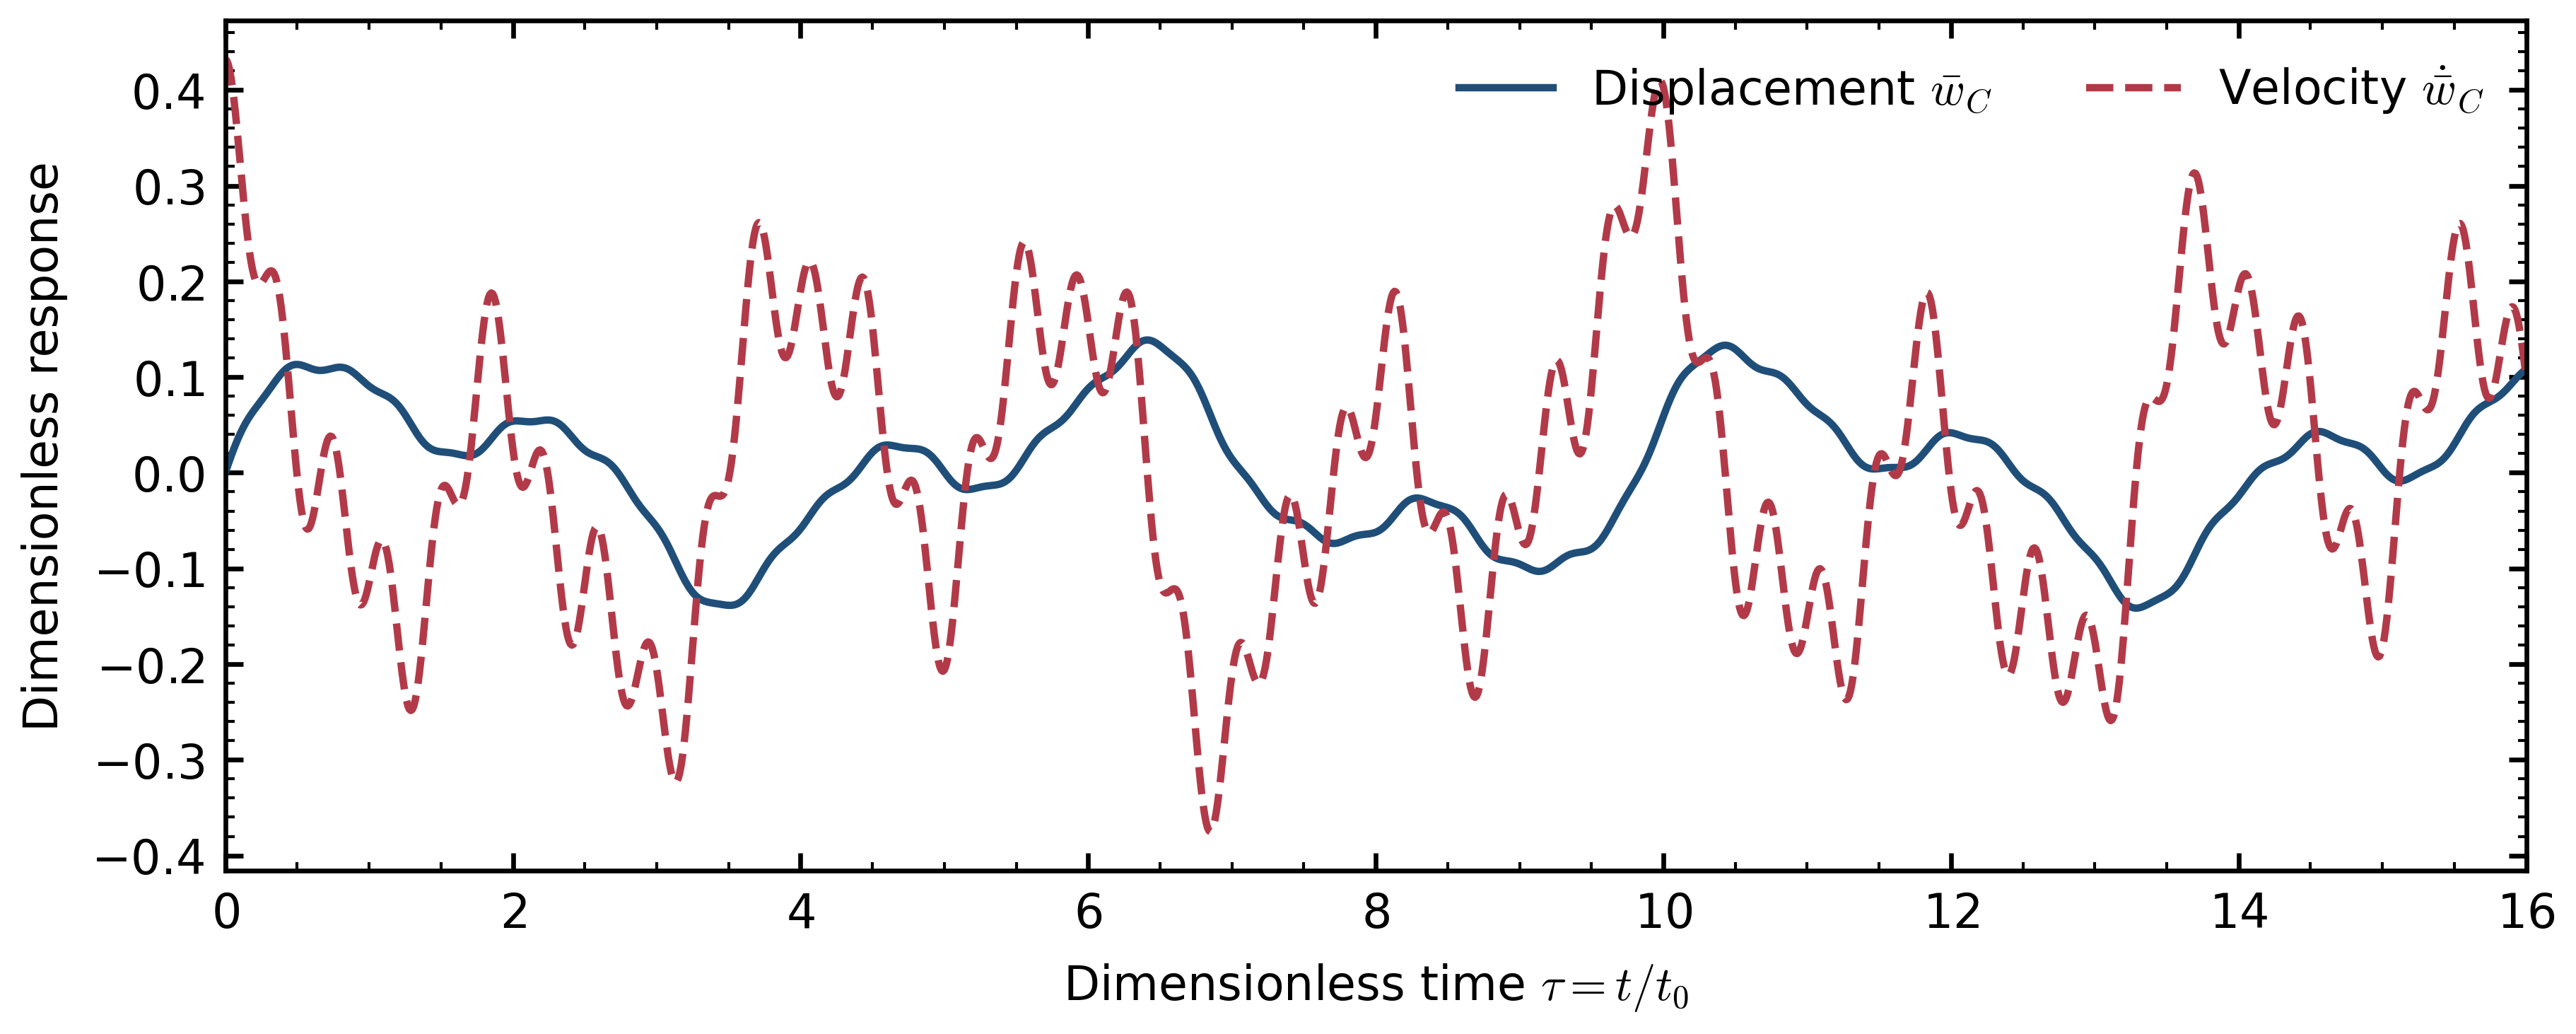
\includegraphics[width=\linewidth]{q3_c_point_response.png}
  \end{columns}
  \takeaway{$C$ 点响应最能体现集中质量初始速度激励的作用。}
\end{frame}

% 16
\begin{frame}{解析全梁时空响应}
  \begin{columns}[T,onlytextwidth]
    \column{0.66\linewidth}
    \centering
    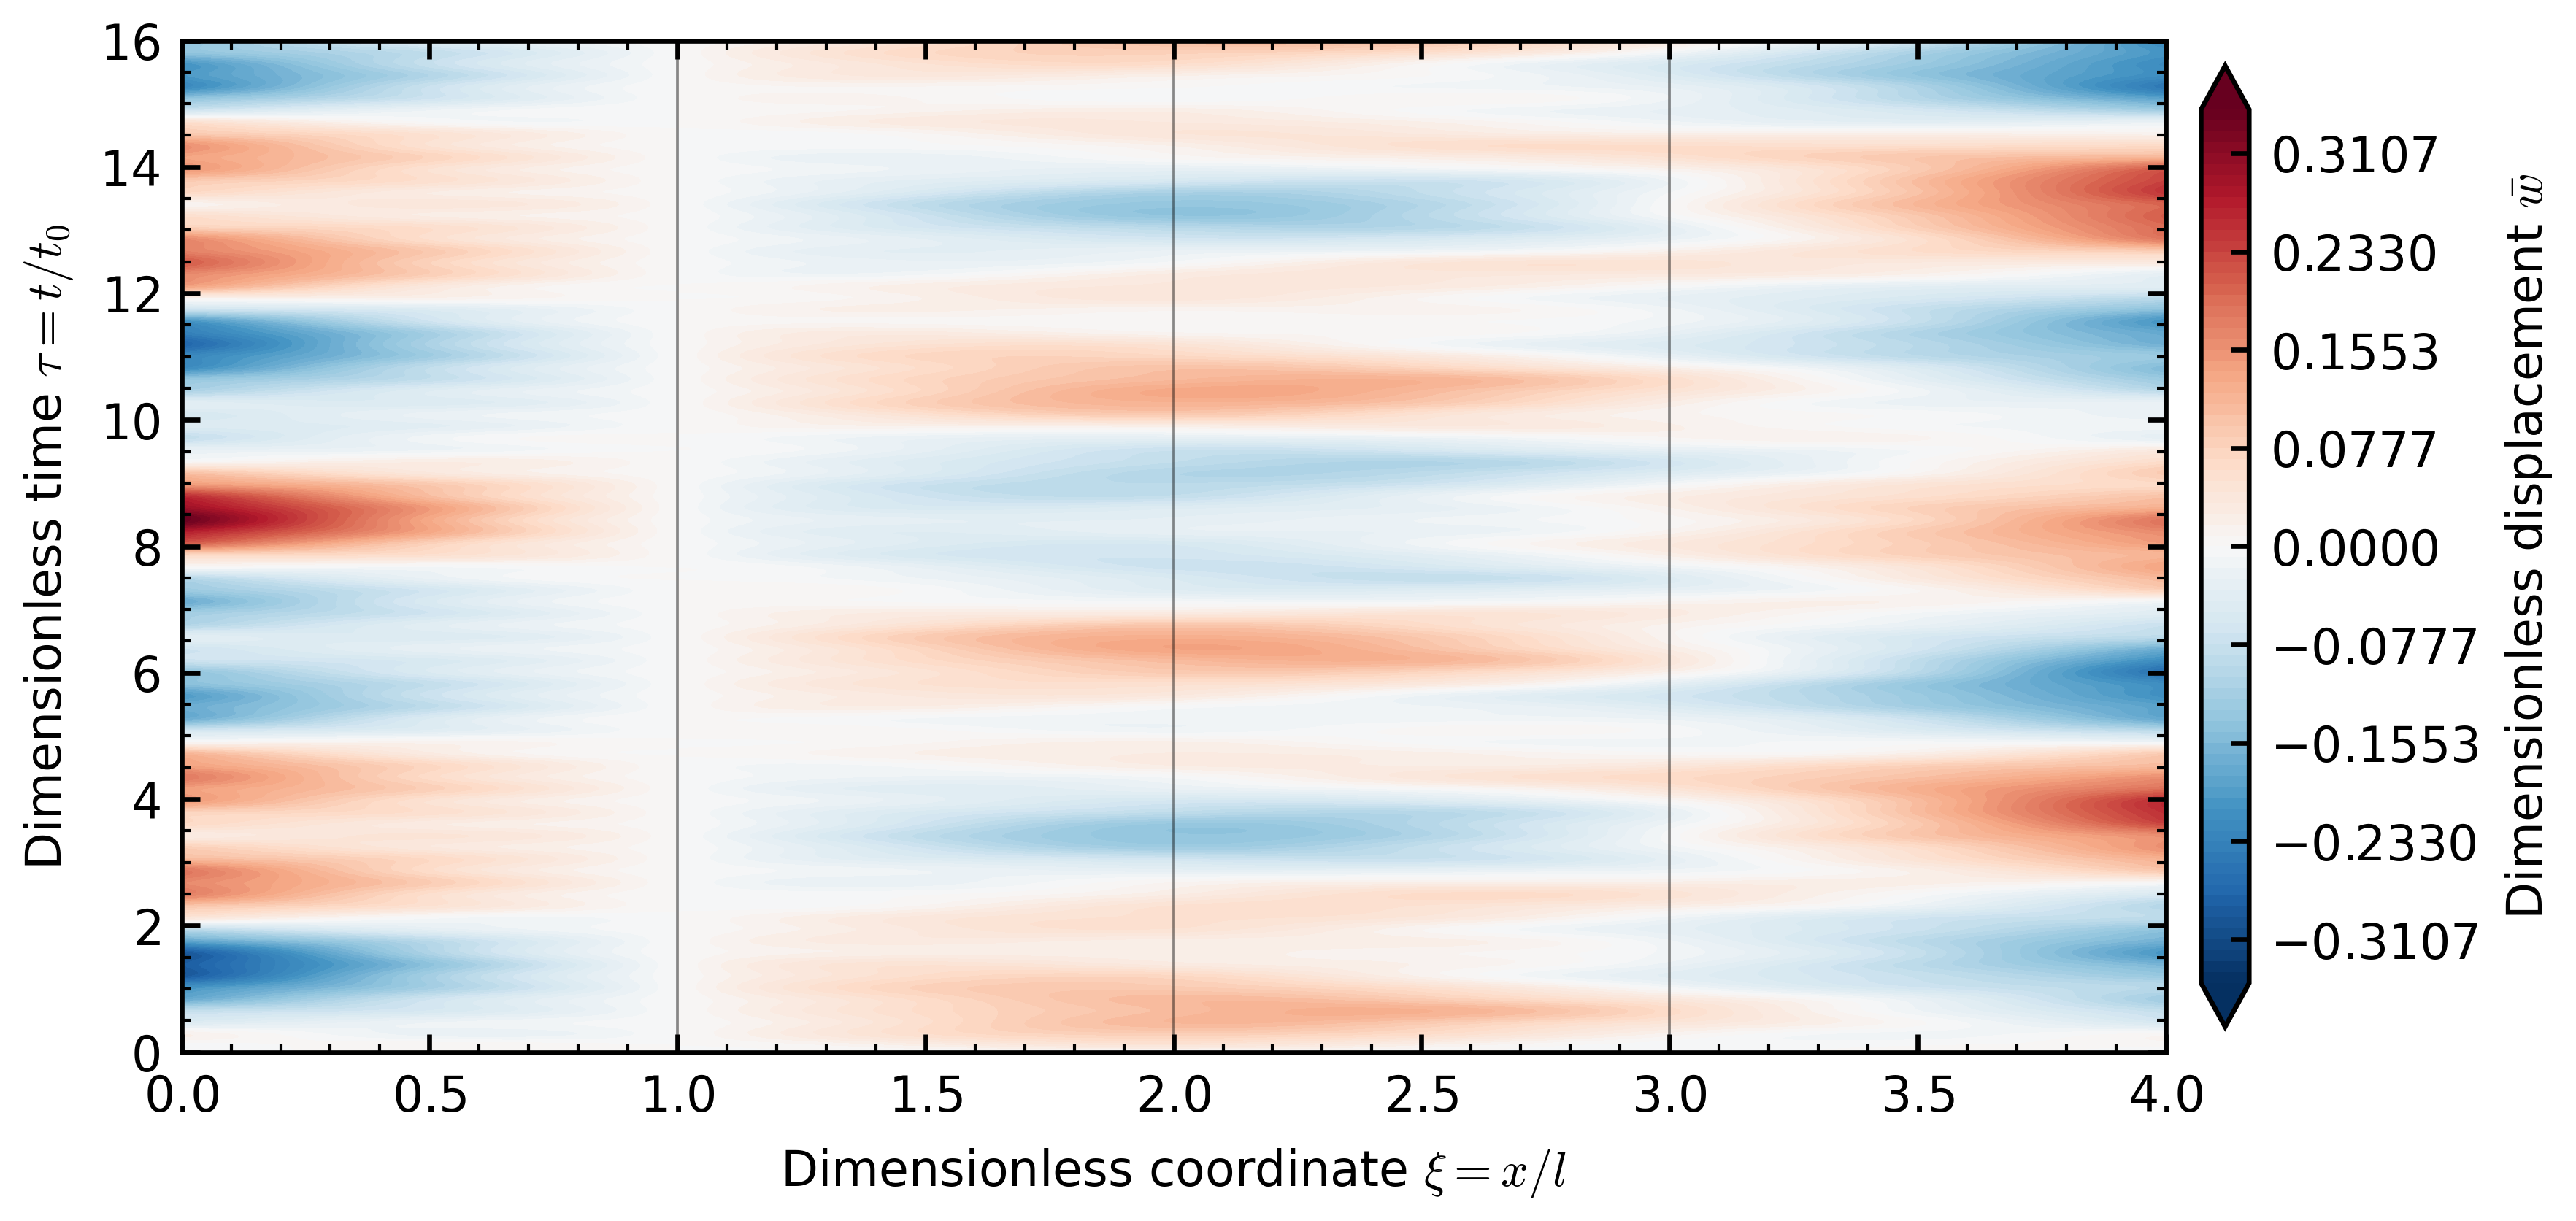
\includegraphics[width=\linewidth]{q3_spacetime_response.png}
    \column{0.30\linewidth}
    \begin{itemize}
      \item 横轴：$\xi=x/l$
      \item 纵轴：$\tau=t/t_0$
      \item 颜色：无量纲位移
      \item 反映全梁响应演化
    \end{itemize}
  \end{columns}
\end{frame}

% 17
\begin{frame}{有限元模型}
  \begin{block}{二节点 Euler--Bernoulli Hermite 梁单元}
    每个节点两个自由度：
    \[
    \{w,\theta\}
    \]
  \end{block}
  \begin{block}{单元刚度矩阵}
    \[
    \mathbf k_e=
    \frac{EJ}{h^3}
    \begin{bmatrix}
    12&6h&-12&6h\\
    6h&4h^2&-6h&2h^2\\
    -12&-6h&12&-6h\\
    6h&2h^2&-6h&4h^2
    \end{bmatrix}
    \]
  \end{block}
\end{frame}

% 18
\begin{frame}{局部构件的有限元处理}
  \begin{columns}[T,onlytextwidth]
    \column{0.52\linewidth}
    \begin{itemize}
      \item $B$ 点：消元法施加 $w_B=0$，保留转角自由度。
      \item $C$ 点：集中质量加入节点平动质量项。
      \item $D$ 点：弹簧刚度加入节点平动刚度项。
      \item 单元数 $N_e=80$，节点数 $81$。
    \end{itemize}
    \column{0.42\linewidth}
    \begin{block}{广义特征值问题}
      \[
      \mathbf K\boldsymbol\Phi_n
      =
      \omega_n^2
      \mathbf M\boldsymbol\Phi_n
      \]
    \end{block}
    \begin{block}{响应}
      前 $24$ 阶模态叠加
    \end{block}
  \end{columns}
\end{frame}

% 19
\begin{frame}{程序与数据流程}
  \begin{center}
    \begin{tikzpicture}[node distance=1.15cm, every node/.style={draw, rounded corners, align=center, minimum width=2.6cm, minimum height=0.8cm}]
      \node (f) {Fortran\\FEM 求解};
      \node[right=of f] (c) {CSV\\数据导出};
      \node[right=of c] (p) {Python\\后处理};
      \node[right=of p] (s) {SciencePlots\\可视化};
      \draw[->,thick] (f) -- (c);
      \draw[->,thick] (c) -- (p);
      \draw[->,thick] (p) -- (s);
    \end{tikzpicture}
  \end{center}
  \vspace{0.6em}
  \begin{columns}[T,onlytextwidth]
    \column{0.5\linewidth}
    \begin{itemize}
      \item \texttt{fem\_frequencies.csv}
      \item \texttt{fem\_modes.csv}
      \item \texttt{fem\_c\_response.csv}
    \end{itemize}
    \column{0.5\linewidth}
    \begin{itemize}
      \item \texttt{fem\_snapshots.csv}
      \item \texttt{frequency\_comparison.csv}
    \end{itemize}
  \end{columns}
  \takeaway{完整流程可复现，不依赖手工整理图表。}
\end{frame}

% 20
\begin{frame}{固有频率对比}
  \begin{columns}[T,onlytextwidth]
    \column{0.62\linewidth}
    \centering
    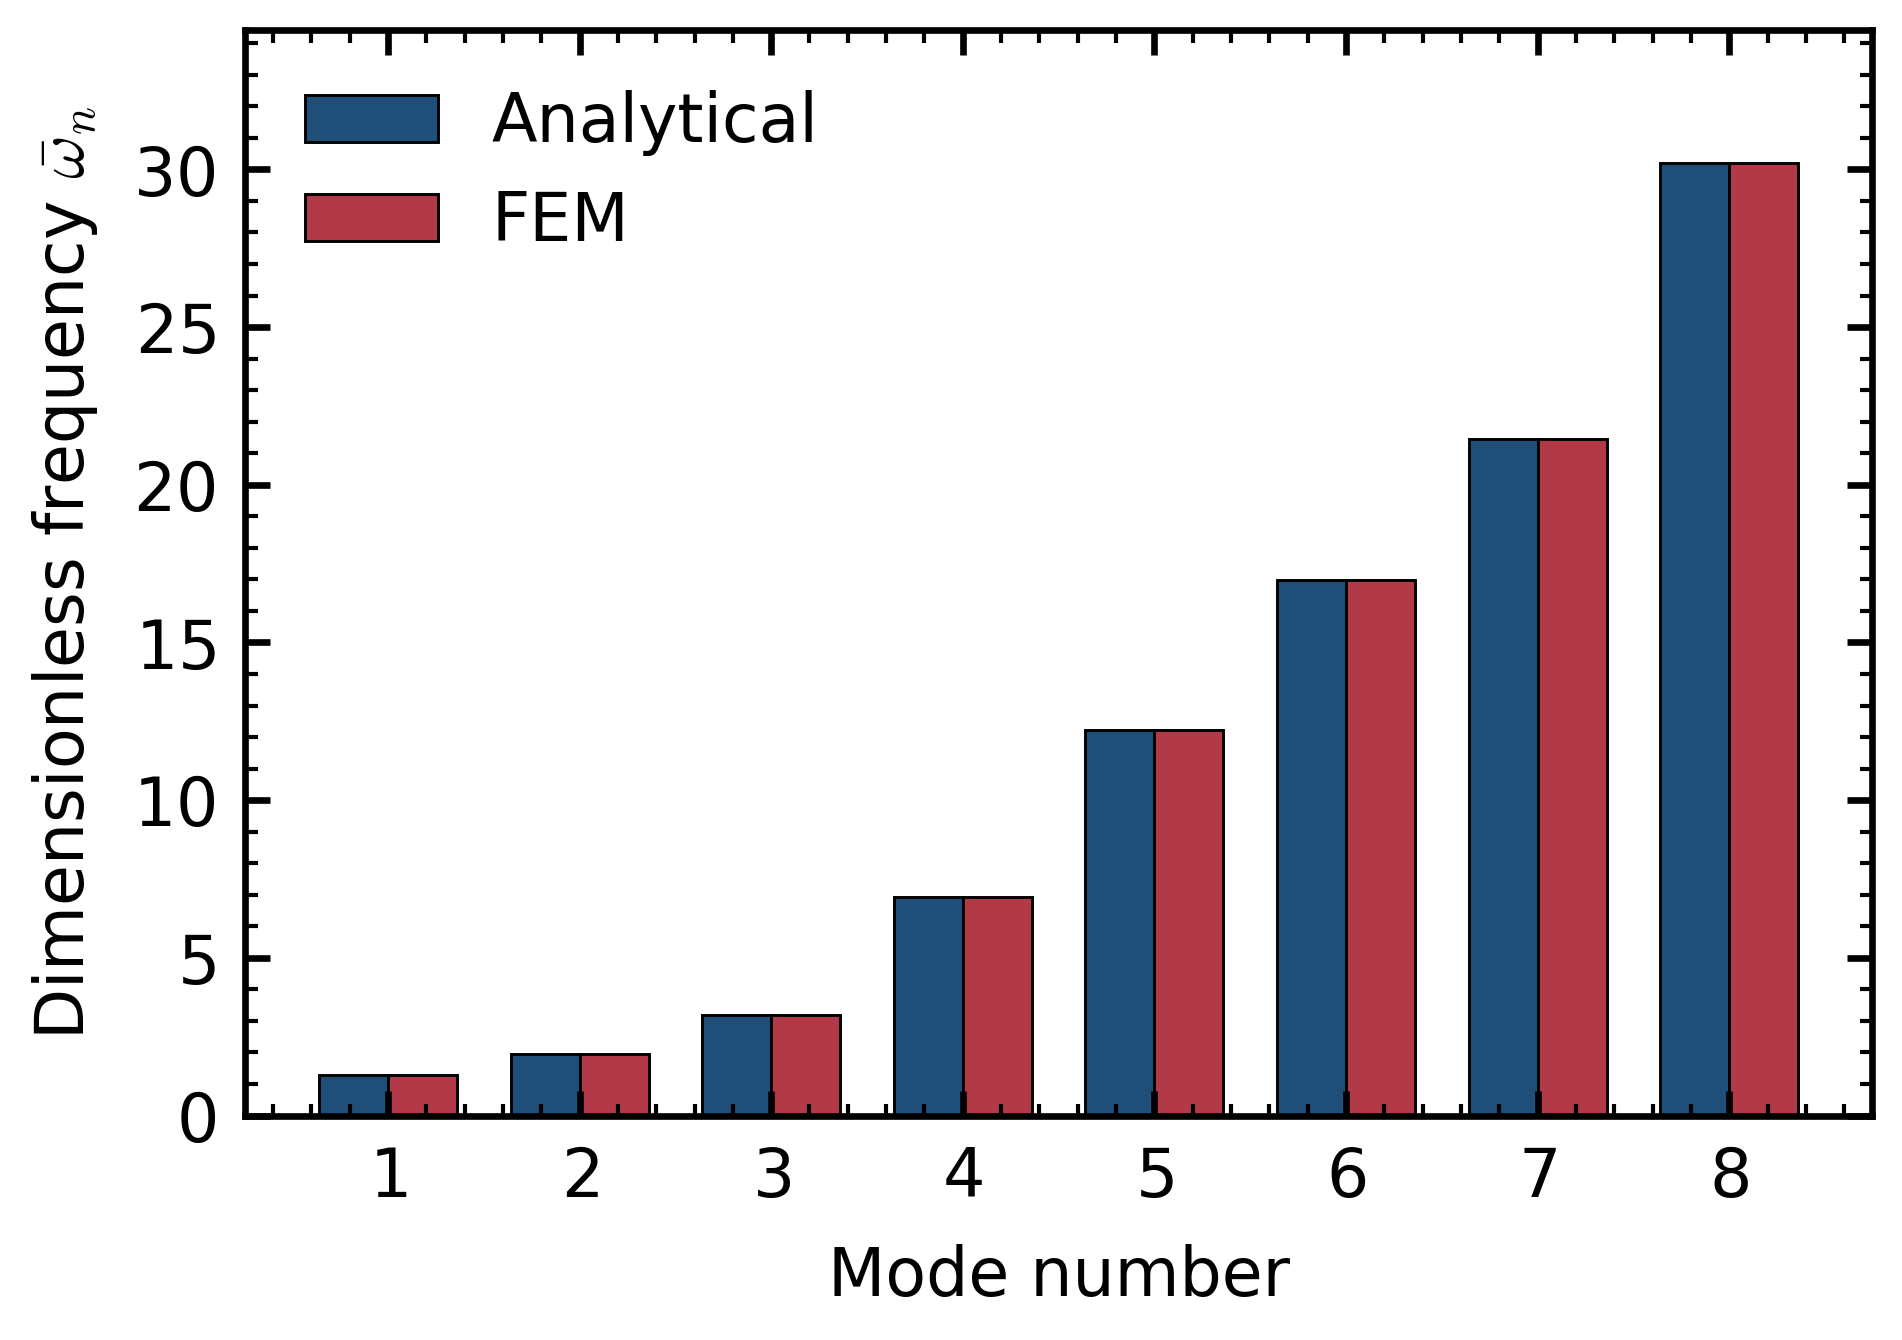
\includegraphics[width=\linewidth]{comparison_frequency_spectrum.png}
    \column{0.34\linewidth}
    \begin{itemize}
      \item 前 8 阶频率几乎重合
      \item 前 11 阶误差较小
      \item 第 12 阶误差增大
      \item 高阶模态开始受空间离散影响
    \end{itemize}
  \end{columns}
  \takeaway{频率对比是模型正确性的第一层证据。}
\end{frame}

% 21
\begin{frame}{频率误差分析}
  \begin{columns}[T,onlytextwidth]
    \column{0.62\linewidth}
    \centering
    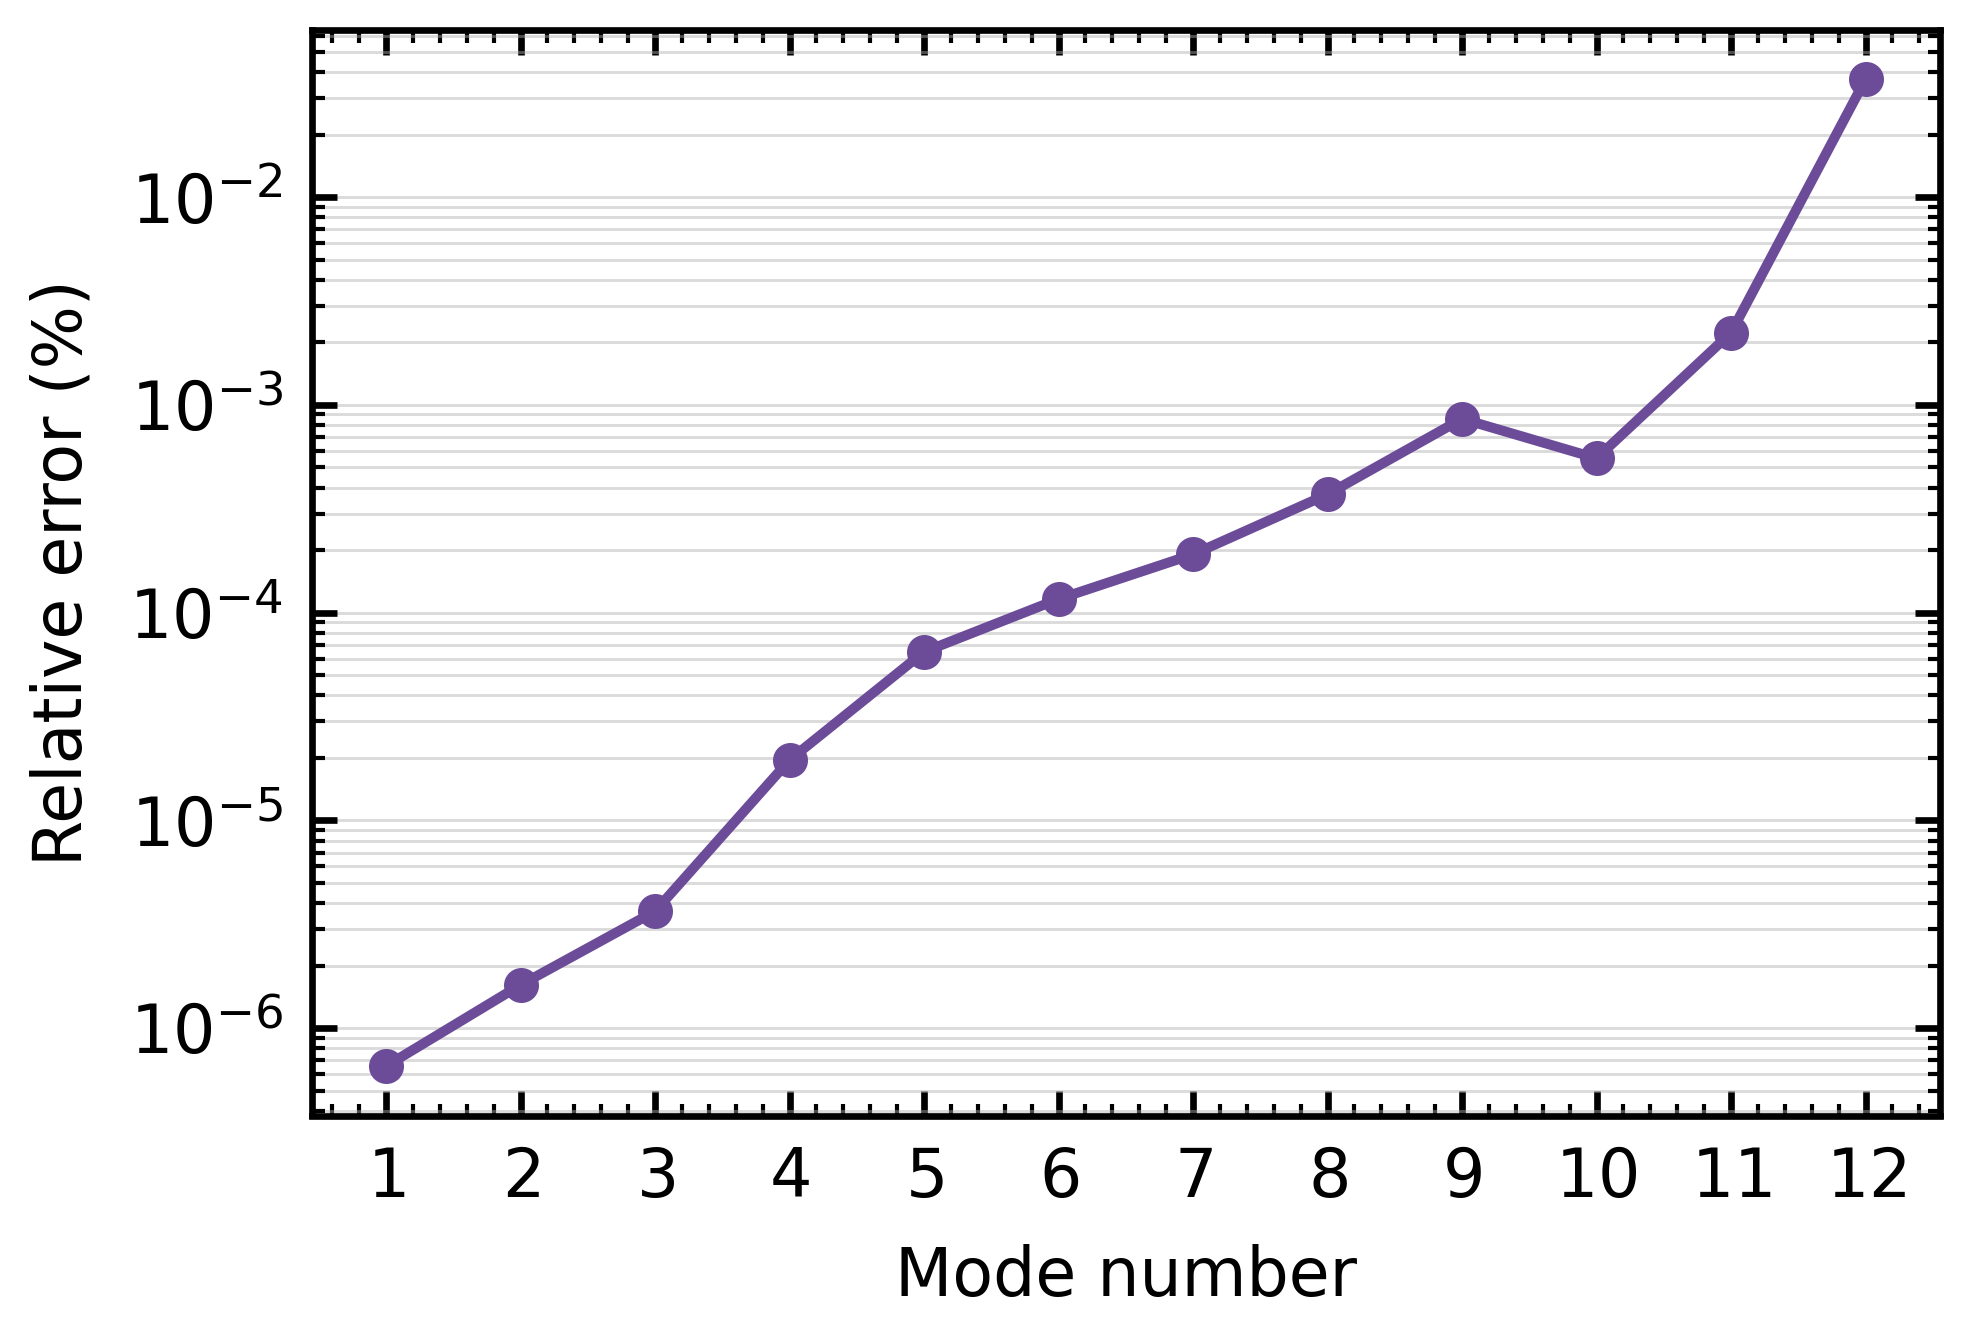
\includegraphics[width=\linewidth]{comparison_frequency_error.png}
    \column{0.34\linewidth}
    \begin{itemize}
      \item 低阶频率误差极小
      \item 误差随阶数总体增大
      \item 高阶误差来自空间离散
      \item 更密网格可改善高阶结果
    \end{itemize}
  \end{columns}
\end{frame}

% 22
\begin{frame}{振型对比}
  \begin{columns}[T,onlytextwidth]
    \column{0.68\linewidth}
    \centering
    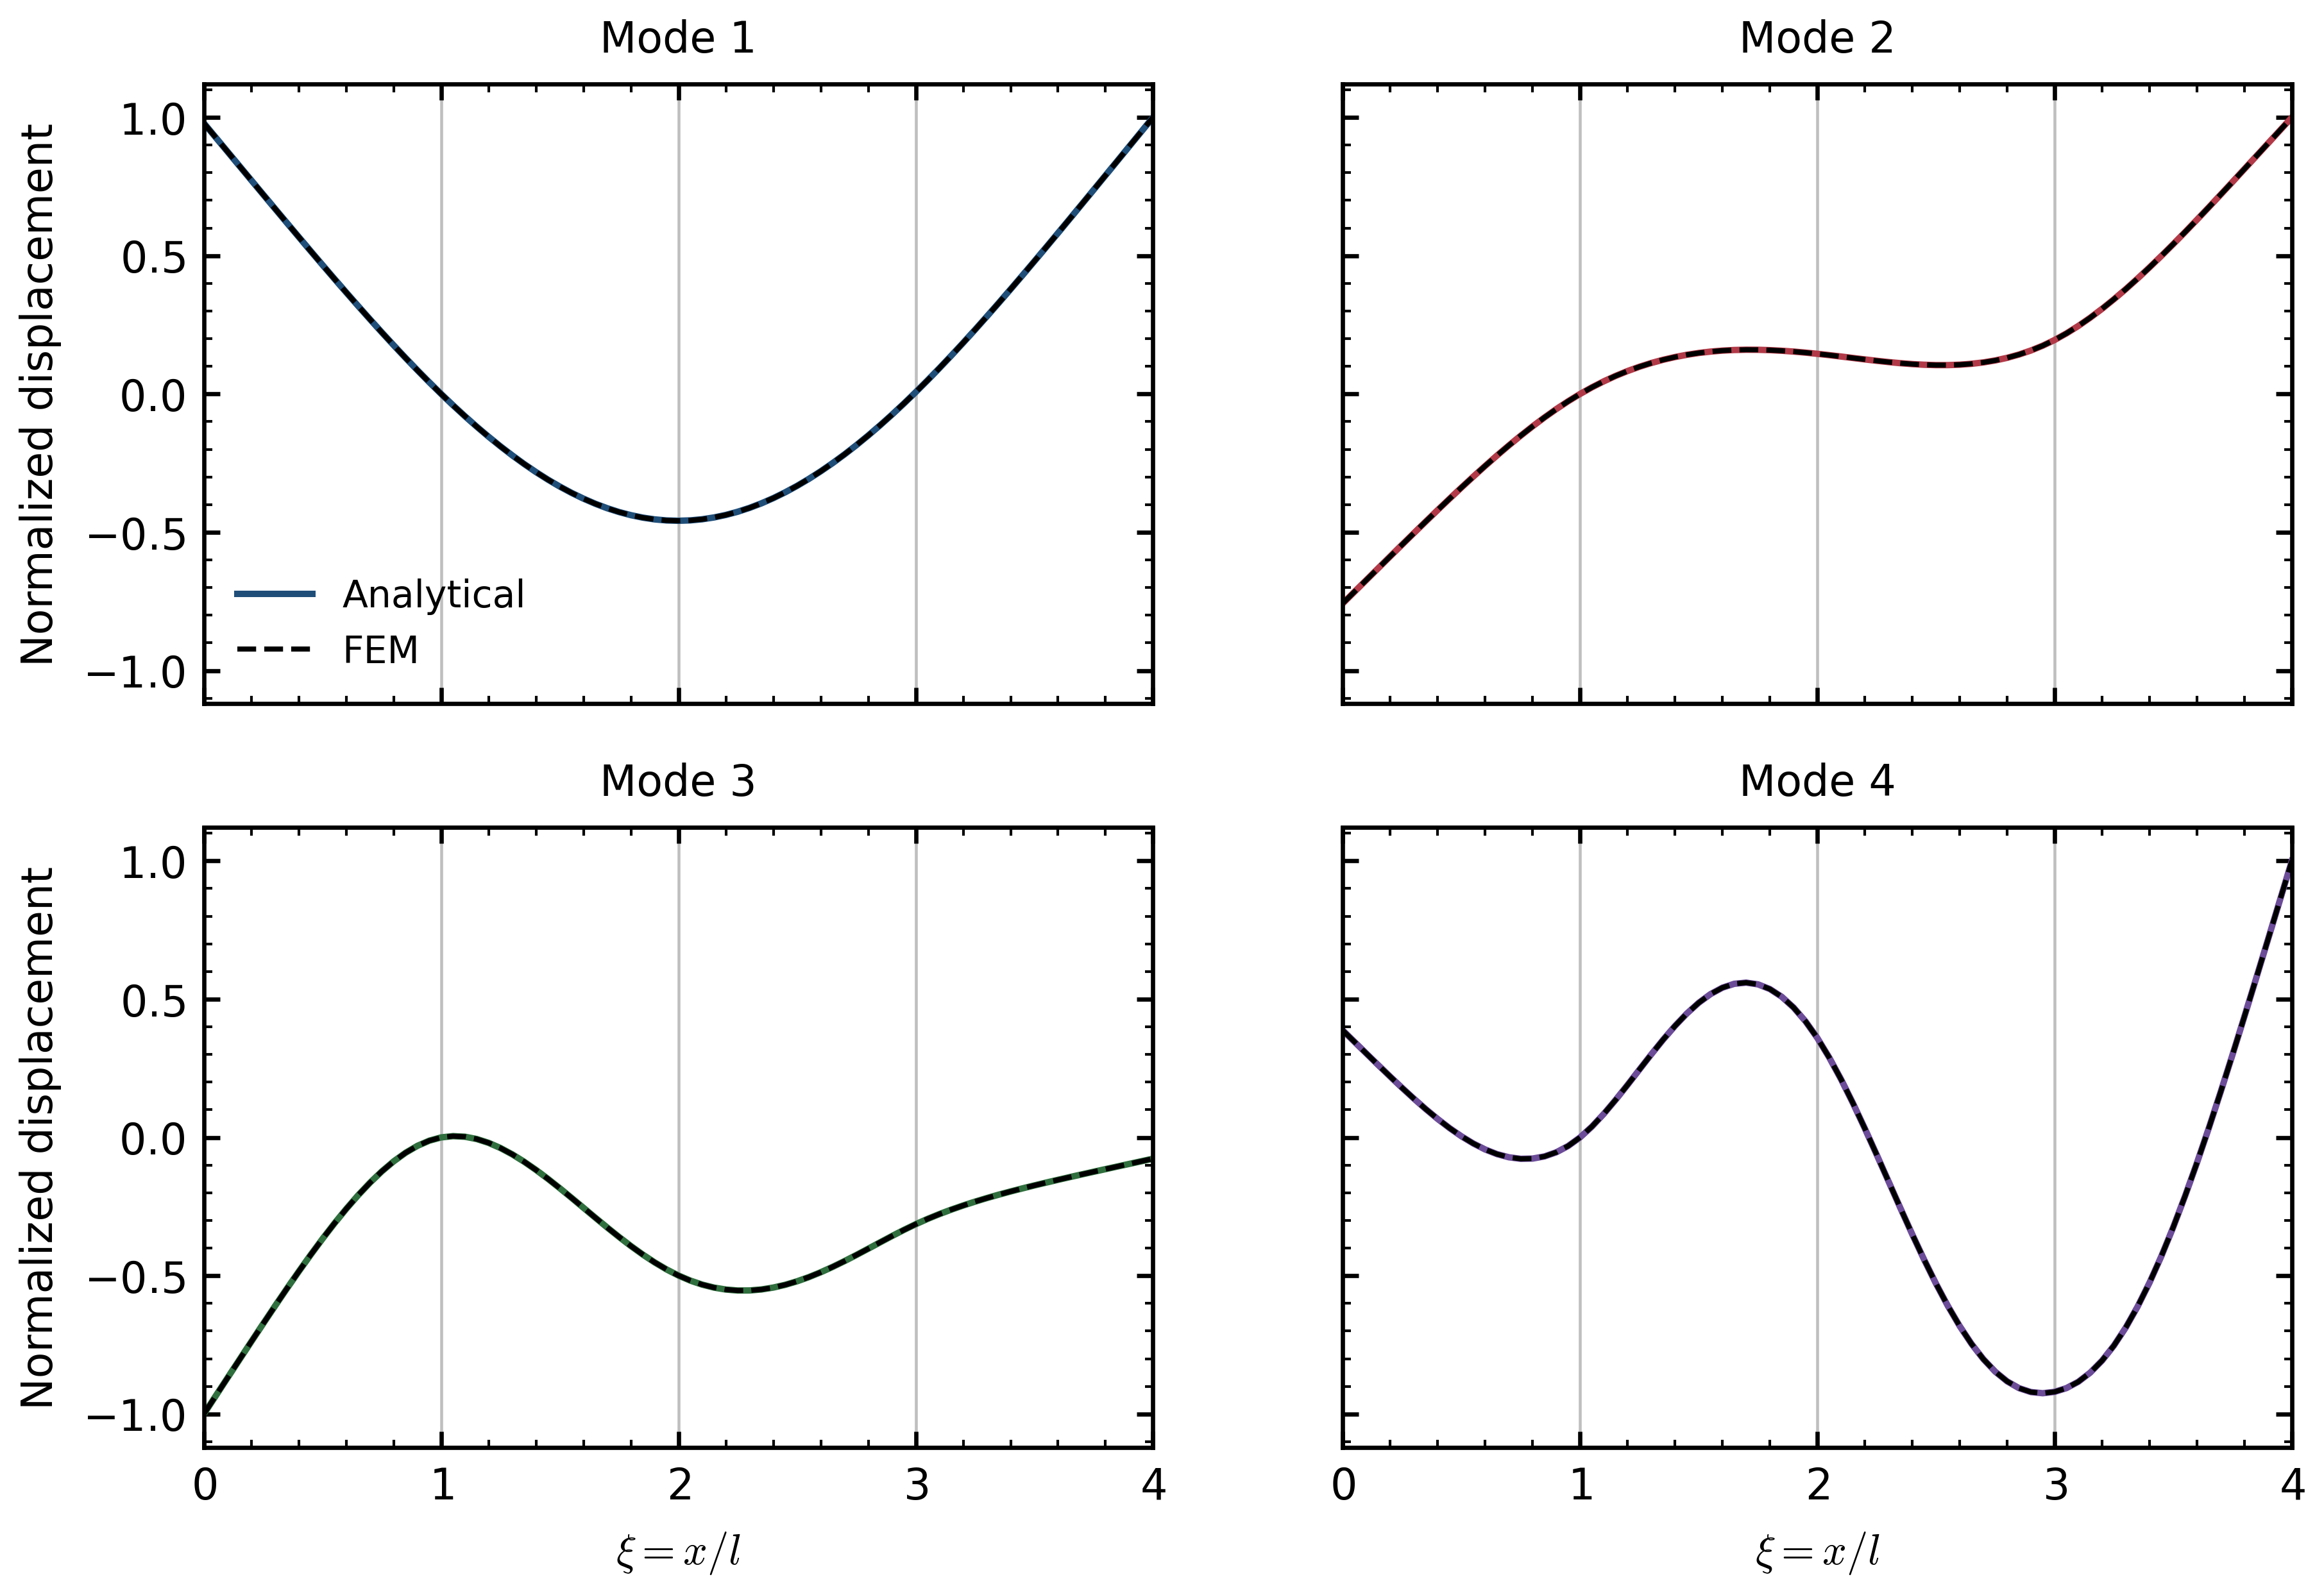
\includegraphics[width=\linewidth]{comparison_mode_overlay.png}
    \column{0.28\linewidth}
    \small
    \begin{itemize}
      \item FEM 振型与解析振型几乎完全重合。
      \item 前四阶节点 $L_2$ 相对误差约为 $10^{-9}$ 至 $10^{-8}$。
    \end{itemize}
  \end{columns}
\end{frame}

% 23
\begin{frame}{动力响应对比与结论}
  \begin{columns}[T,onlytextwidth]
    \column{0.58\linewidth}
    \centering
    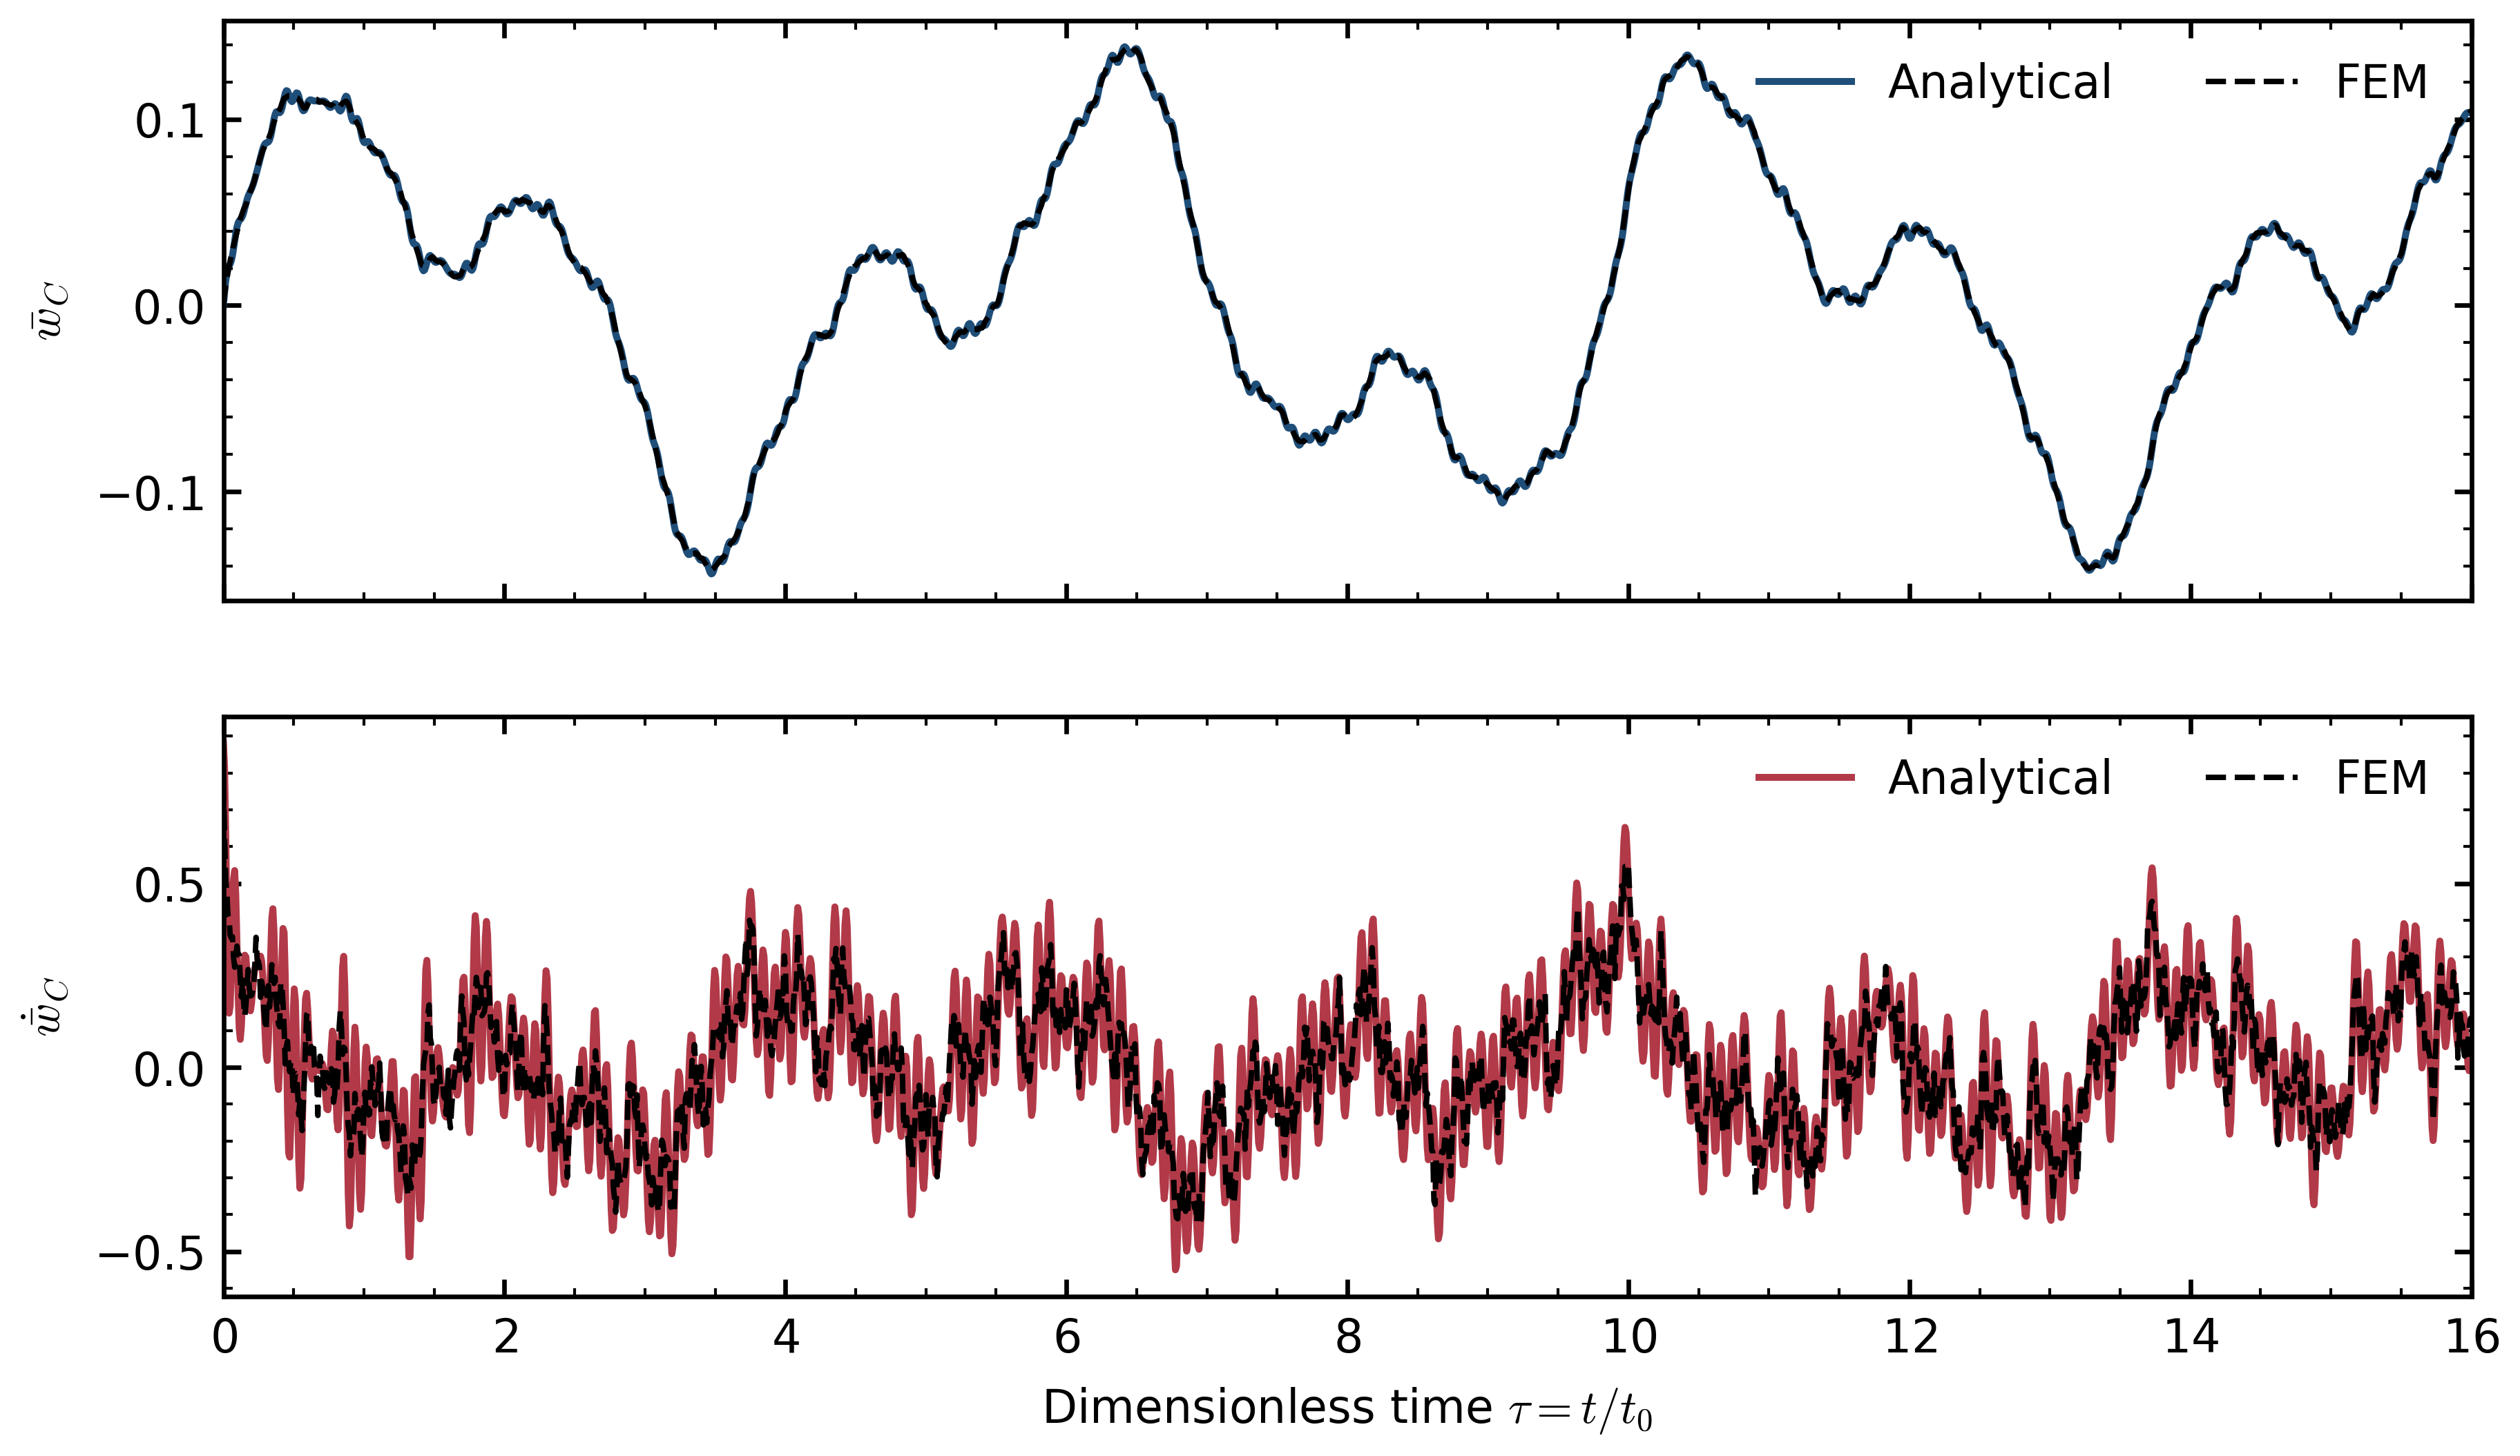
\includegraphics[width=\linewidth]{comparison_c_response.png}
    \column{0.38\linewidth}
    \begin{enumerate}
      \item 传递矩阵法可有效处理状态跳跃。
      \item FEM 能准确复现低阶频率与振型。
      \item 位移响应吻合较好。
      \item 速度响应对高阶模态更敏感。
    \end{enumerate}
  \end{columns}
  \vspace{0.4em}
  \begin{block}{展望}
    增加单元数；研究不同 $\alpha,\kappa$；扩展到阻尼和强迫振动。
  \end{block}
\end{frame}

\end{document}
